\documentclass[11pt,a4paper]{article}
\usepackage[paperwidth=210mm,paperheight=520mm,margin=1.5cm]{geometry}
\usepackage{graphicx}
\usepackage{float}

% Kill the effing page number!
\pagestyle{empty}
\makeatletter
\let\ps@plain\ps@empty
\makeatother


\title{Exercise 2: Uncertainty Prediction}
\author{}
\date{}

\begin{document}

\maketitle

This document shows the implementation of error estimation for a CNN model trained on the GALAH star spectra dataset. 
The model was used to predict the three labels $t\_eff$, $log\_g$, and $fe\_h$.

\section*{Result Plots}

\begin{figure}[H]
    \centering
    \begin{minipage}{0.48\linewidth}
        \centering
        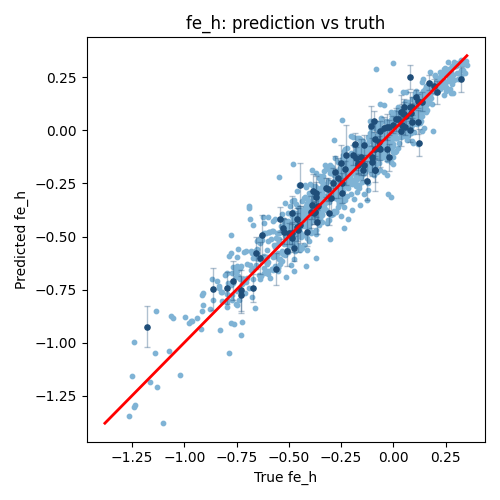
\includegraphics[width=\linewidth]{../fe_h_pred_vs_true_uncertainty.png}
    \end{minipage}
    \hfill
    \begin{minipage}{0.48\linewidth}
        \centering
        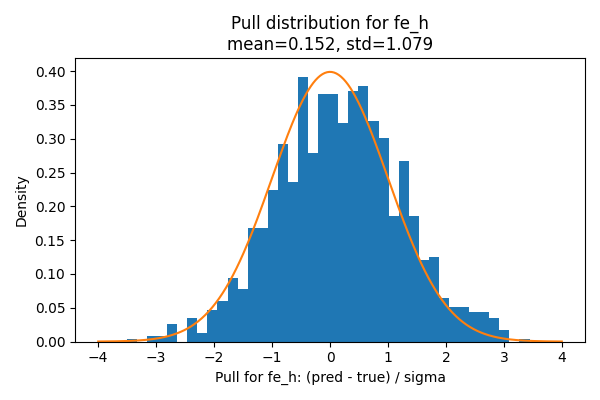
\includegraphics[width=\linewidth]{../fe_h_pull_distribution.png}
    \end{minipage}
    \caption{Results for metallicity, $\mathrm{[Fe/H]}$. Left: predicted versus true values with a subset of values with representative uncertainty bars and the red diagonal indicating perfect agreement. Right: pull distribution for $\mathrm{[Fe/H]}$, compared to the standard normal distribution to assess uncertainty calibration.}
    \label{fig:feh-results}
\end{figure}

\begin{figure}[H]
    \centering
    \begin{minipage}{0.48\linewidth}
        \centering
        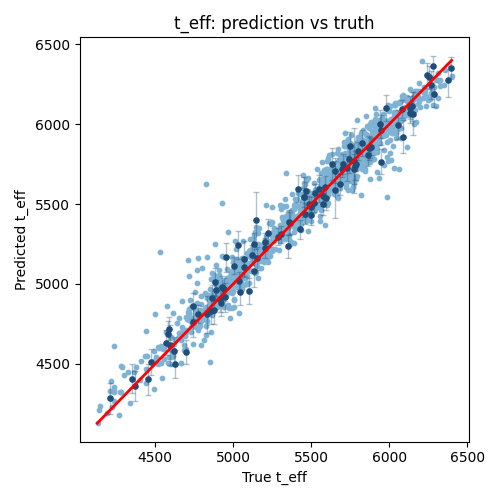
\includegraphics[width=\linewidth]{../t_eff_pred_vs_true_uncertainty.png}
    \end{minipage}
    \hfill
    \begin{minipage}{0.48\linewidth}
        \centering
        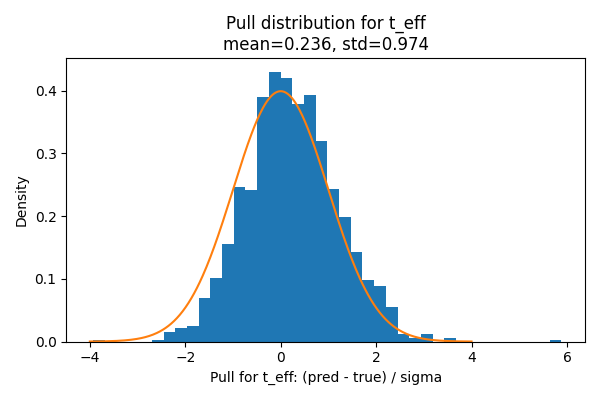
\includegraphics[width=\linewidth]{../t_eff_pull_distribution.png}
    \end{minipage}
    \caption{Results for effective temperature, $T_{\mathrm{eff}}$. Left: predicted versus true values with a subset of values with representative uncertainty bars and the red diagonal indicating perfect agreement. Right: pull distribution for $T_{\mathrm{eff}}$, compared to the standard normal distribution to assess uncertainty calibration.}
    \label{fig:teff-results}
\end{figure}

\begin{figure}[H]
    \centering
    \begin{minipage}{0.48\linewidth}
        \centering
        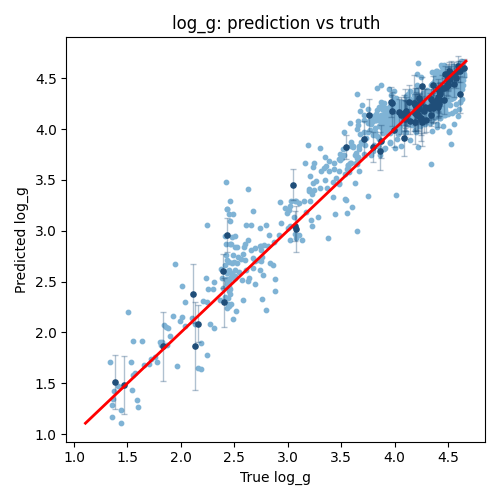
\includegraphics[width=\linewidth]{../log_g_pred_vs_true_uncertainty.png}
    \end{minipage}
    \hfill
    \begin{minipage}{0.48\linewidth}
        \centering
        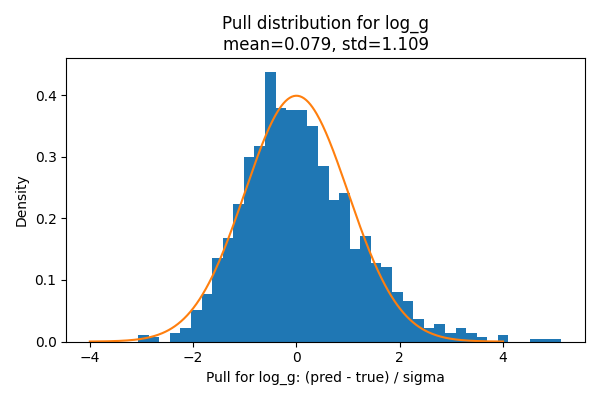
\includegraphics[width=\linewidth]{../log_g_pull_distribution.png}
    \end{minipage}
    \caption{Results for surface gravity, $\log g$. Left: predicted versus true values with a subset of values with representative uncertainty bars and the red diagonal indicating perfect agreement. Right: pull distribution for $\log g$, compared to the standard normal distribution to assess uncertainty calibration.}
    \label{fig:logg-results}
\end{figure} 

\begin{figure}[H]
    \centering
    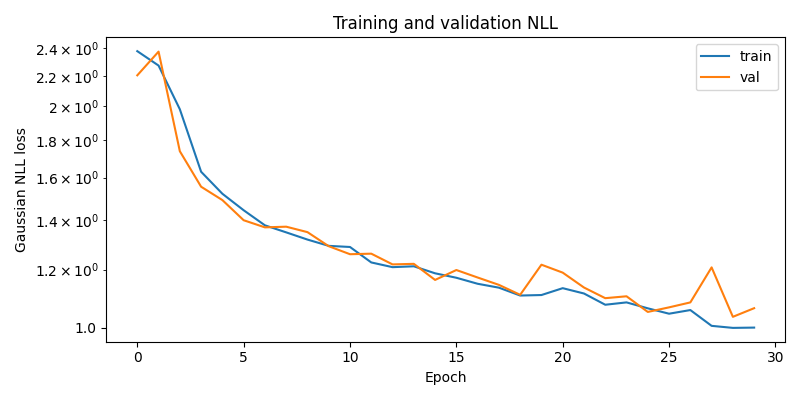
\includegraphics[width=0.72\linewidth]{../loss_curve_uncertainty.png}
    \caption{Training and validation NLL (negative log-likelihood) during training. Both curves decrease in a similar way, which suggests stable learning without strong overfitting.}
    \label{fig:nll-loss}
\end{figure}


\end{document}
